\let\negmedspace\undefined
\let\negthickspace\undefined
\documentclass[journal]{IEEEtran}
\usepackage[a5paper, margin=10mm, onecolumn]{geometry}
%\usepackage{lmodern} % Ensure lmodern is loaded for pdflatex
\usepackage{tfrupee} % Include tfrupee package

\setlength{\headheight}{1cm} % Set the height of the header box
\setlength{\headsep}{0mm}     % Set the distance between the header box and the top of the text

\usepackage{gvv-book}
\usepackage{gvv}
\usepackage{cite}
\usepackage{amsmath,amssymb,amsfonts,amsthm}
\usepackage{algorithmic}
\usepackage{graphicx}
\usepackage{textcomp}
\usepackage{xcolor}
\usepackage{txfonts}
\usepackage{listings}
\usepackage{enumitem}
\usepackage{mathtools}
\usepackage{gensymb}
\usepackage{comment}
\usepackage[breaklinks=true]{hyperref}
\usepackage{tkz-euclide} 
\usepackage{listings}
% \usepackage{gvv}                                        
\def\inputGnumericTable{}                                 
\usepackage[latin1]{inputenc}                                
\usepackage{color}                                            
\usepackage{array}                                            
\usepackage{longtable}                                       
\usepackage{calc}                                             
\usepackage{multirow}                                         
\usepackage{hhline}                                           
\usepackage{ifthen}                                           
\usepackage{lscape}
\begin{document}
\bibliographystyle{IEEEtran}
\title{4.9.4}
\author{EE25BTECH11002 - Achat Parth Kalpesh }
{\let\newpage\relax\maketitle}
\renewcommand{\thefigure}{\theenumi}
\renewcommand{\thetable}{\theenumi}
\setlength{\intextsep}{10pt} % Space between text and floats
\numberwithin{equation}{enumi}
\numberwithin{figure}{enumi}
\renewcommand{\thetable}{\theenumi}
\parindent 0px


\textbf{Question:}\\
 The equations of the lines which pass through the point \brak{3, -2} and are inclined at $60\degree$ to the line $\sqrt{3} x+y=1$ is
\begin{enumerate}
\item $y+2=0$, $\sqrt{3}x-y-2-3\sqrt{3}=0$
\item $x-2=0$, $\sqrt{3}x-y+2+3\sqrt{3}=0$
\item $\sqrt{3}x-y-2-3\sqrt{3}=0$
\item None of these
\end{enumerate}

\textbf{Solution:}\\
The given line can be written in normal form as
\begin{align}
    \vec{n}_1^\top \vec{x} = 1,
\end{align}
where
\begin{align}
    \vec{n}_1 = \myvec{\sqrt{3}\\1}, \quad \vec{x} = \myvec{x\\y}.
\end{align}
Let the required line have normal vector $\vec{n}=\myvec{-m\\1}$, where m is the slope of line,then its equation is
\begin{align}
    \vec{n}^\top \vec{x} = c.
\end{align}
Since the line passes through $\vec{P}=\myvec{3\\-2}$,
\begin{align}
     \vec{n}^\top \vec{P} = c
\end{align}


The angle $\theta$ between two lines is given as;
\begin{align}
    \cos\theta = \frac{\vec{n}_1^\top \vec{n}}{\norm{\vec{n}_1}\norm{\vec{n}}}.
\end{align}
Here $\theta = $60\degree$ \implies \cos\theta = \frac{1}{2}$, so
\begin{align}
    \brak{\vec{n}_1^\top \vec{n}}^2 = \frac{1}{4}\norm{\vec{n}_1}^2 \norm{\vec{n}}^2.
\end{align}
Substituting values:
\begin{align}
    \brak{-\sqrt{3}m + 1}^2 &= \frac{1}{4}\brak{4}\brak{\brak{-m}^2+1^2}\\
    \brak{-\sqrt{3}m + 1}^2 &= m^2 + 1^2\\
    3m^2 - 2\sqrt{3}m + 1 &= m^2 + 1, \\
    2m^2 &= 2\sqrt{3}m  \\
    m = 0 \text{ or } m &= \sqrt{3}
\end{align}

For m = 0 ;
\begin{align}
    \vec{n} &= \myvec{0\\1}\\
    \vec{n}^\top \vec{P} &= c
\end{align}
\begin{align}
    c = \myvec{0&1}\myvec{3\\-2}&=-2,
\end{align}
so the line is
\begin{align}
    y+2=0
\end{align}

For m = $\sqrt{3}$ ;
\begin{align}
\vec{n} &= \myvec{-\sqrt{3}\\1}\\
\vec{n}^\top \vec{P} &= c
\end{align}
\begin{align}
    c = \myvec{-\sqrt{3}&1}\myvec{3\\-2} &= -3\sqrt{3}-2
\end{align}
so the line is
\begin{align}
     \sqrt{3}x - y - 3\sqrt{3}-2 = 0
\end{align}

\begin{figure}[h!]
    \centering
    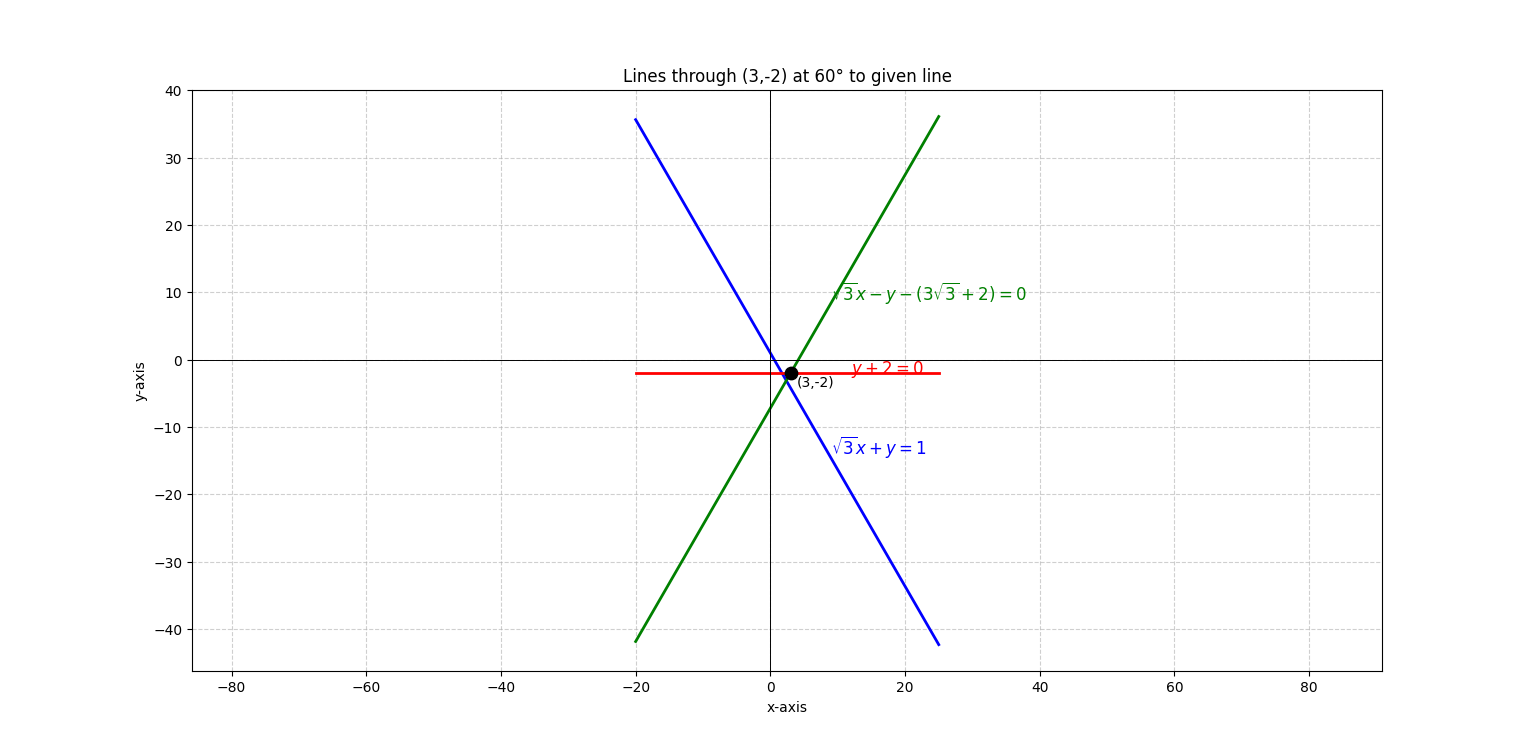
\includegraphics[width=0.655\columnwidth]{figs/pure_python.png}
    \caption{Lines through \brak{3,-2} at 60\degree to given line}
    \label{fig:fig}
 \end{figure}

\end{document}


